\documentclass{article}
\usepackage{amsmath}
\usepackage{graphicx}
\usepackage{mdframed}
\usepackage[dvipsnames]{xcolor}
\usepackage[colorlinks=true,urlcolor=ForestGreen]{hyperref}
\newcommand{\dspace}{\baselineskip 16pt}
\newcommand{\sspace}{\baselineskip 14pt}
\textheight 9in
\textwidth 6.5in 
\oddsidemargin -0.1in \evensidemargin -0.1in
\topmargin -0.3in
\pagestyle{empty}


\newcounter{problem}[section]
\newenvironment{problem}[1][]{\refstepcounter{problem}\par\medskip
   \noindent \textbf{Problem~\theproblem. #1} \rmfamily}{\medskip}
\newcounter{task}[section]
\newenvironment{task}[1][]{\refstepcounter{task}\par\medskip
   \noindent \textbf{Task~\thetask. #1} \rmfamily}{\medskip}
\newenvironment{proof}{\begin{mdframed}\textbf{Ans:}}{ \end{mdframed}}


\begin{document}
\sspace
\noindent
Purdue University \hfill Duc Viet Le\\
CS 59000SA        \hfill 
% \href{mailto:le52@purdue.edu}{le52@purdue.edu}
\dspace
\begin{center}
{\bf Assignment 5}
\end{center}
\vspace{.2in}
\begin{problem} Assume we have a sequence of $t$ inputs, namely $x_1 , x_2 , \dots , x_t$ . Construct neural networks
based on the following requirements. 
\begin{enumerate}
    \item  Draw a feed-forward neural network using A that will perform equivalent computation on the given input as the above RNN. Clearly mark input, output and all connections. Justify your answer.

    \textbf{Answer. }
    This is an equivalent feed-forward neural network using $A$ that will perform equivalent computation. 
    \begin{figure}[h!]
        \centering
        \includegraphics[scale=.7]{fig/feed-forward.png}
        \caption{Equivalent feed-forward neural network using $A$}
    \end{figure}
    \\
    $x_i$ just as input at different time.
    \item To use a feed-forward neural network to simulate a RNN, what weight constraints are needed? What's the space complexity for the model of RNN? What about it's equivalent feed-forward network version?
    \begin{proof}
        The weight has to be the same at every layer. Also,  we want $w_i = w_j$ for all $i\neq j$, and when we updates the weight values, we want the weight changes has to be the same (i.e. $\Delta w_i = \Delta w_j$).

        If $x_i$ is the scalar value, the space complexity $\mathcal O(1)$ for RNN because we only need to store one input at a time. In the equivalent feed-forward network, it will be $\mathcal O(t)$ 

        Otherwise, if $x_i$ is vector (says, size $n$), then it will be $\mathcal O(n)$ for RNN, and $\mathcal O(nt)$ for feed-forward. 
    \end{proof}
\end{enumerate}
\end{problem}

\begin{problem}
In this question, you are going to learn how gradient vanish problem can occur.
\begin{enumerate}
    \item The output range of the sigmoid function is: 
    \begin{proof}
    $(-1,1)^{|h|}$ (vector of length $|h|$, each value in the interval $(-1,1)$). I assume the $tanh(\cdot)$ is the non-linearity functioned used. 
    \end{proof}
    \item Prove why Equation 5.4 can suffer from vanishing gradient or gradient explosion problem
    \begin{proof}
        As explained in the lecture notes, we have:
        \begin{equation}
            ||\frac{\partial{h_i}}{\partial{h_{i-1}}}|| \leq ||W^T||||diag(sigmoid(h_{i+1}))|| \leq \alpha_a\alpha_b
        \end{equation}
        Therefore, in the equation (5.4), the quantity: 
        \begin{equation}
            \bigg|\bigg|\prod^{t}_{k+1}\frac{\partial{h_i}}{\partial{h_{i-1}}}\bigg|\bigg| \leq (\alpha_a\alpha_b)^{t-k}
        \end{equation}
        this quantity can become very large ($\alpha_a\alpha_b > 1$) or very small ($\alpha_a\alpha_b < 1$). Thus, when the gradient value becomes very large, it causes gradient explosion, and when the gradient becomes very small, it causes vanishing gradient.
    \end{proof}
\end{enumerate}
\end{problem}

\begin{problem}
   Sketch the structure of LSTM based on the above description and following equation, clearly mark what's the input and output for each gate.
\end{problem}
\\\textbf{Answer:}
The following figure is the sketched structure of LSTM
   \begin{figure}[h!]
        \centering
        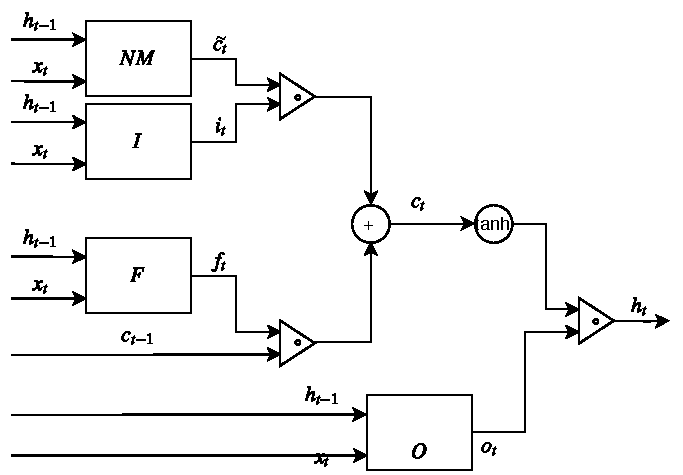
\includegraphics[scale=.7]{fig/LSTM.pdf}
        \caption{Structure of LSTM}
    \end{figure}
\begin{problem}
    Which gate(s) of LSTM help prevent gradient vanishing problem? Justify your answer.
\end{problem}
\begin{proof}
    Forget gate, $f_t = F(x_t ,h_{t-1})$. The idea is that it makes an assessment on wether the past memory cell is useful for the computation of the current memory cell. 
\end{proof}

\begin{problem}
    What's the difference between a memory cell and a memory block?
\end{problem}
\begin{proof}
    LTSM allows the network to memorize information after several timestep, and those memories are stored in memory cell.

    Memory block contains one or more memory cells sharing the same input gate. Memory block of size 1 is the same as a memory cell.
\end{proof}
\end{document}